\documentclass[11pt, letterpaper]{article}

% ----- Packages -----
\usepackage[utf8]{inputenc}
\usepackage{amsmath, amssymb, amsthm, mathrsfs, amsfonts, mathtools}
\usepackage{geometry}
\geometry{margin=1.15in}
\usepackage{hyperref}
\usepackage{xcolor}
\usepackage{titlesec}
\usepackage{enumitem}
\usepackage{authblk}
\usepackage{booktabs}
\usepackage{graphicx}
\usepackage{float}
\usepackage{mdframed}

% ----- Formatting -----
\hypersetup{
    colorlinks=true,
    linkcolor=blue,
    filecolor=magenta,
    urlcolor=blue,
    citecolor=black,
}
\titleformat{\section}{\large\bfseries}{\thesection.}{1em}{}
\titleformat{\subsection}{\normalsize\bfseries}{\thesubsection}{1em}{}

% ----- Math Commands -----
\newcommand{\R}{\mathbb{R}}
\newcommand{\C}{\mathbb{C}}
\newcommand{\Z}{\mathbb{Z}}
\newcommand{\N}{\mathbb{N}}
\newcommand{\G}{G^*}
\newcommand{\PT}{\mathcal{PT}}
\newcommand{\Man}{\mathcal{M}}
\newcommand{\Hilb}{\mathcal{H}}
\newcommand{\Lag}{\mathcal{L}}
\DeclareMathOperator{\ReOp}{Re}
\DeclareMathOperator{\ImOp}{Im}
\DeclareMathOperator{\Tr}{Tr}
\DeclareMathOperator{\sgn}{sgn}
\DeclareMathOperator{\Sp}{Softplus}
\DeclareMathOperator{\Spec}{Spec}

% ----- Theorem Environments -----
\newtheorem{theorem}{Theorem}[section]
\newtheorem{lemma}[theorem]{Lemma}
\newtheorem{corollary}[theorem]{Corollary}
\newtheorem{proposition}[theorem]{Proposition}
\theoremstyle{definition}
\newtheorem{definition}{Definition}[section]
\newtheorem{example}[theorem]{Example}
\theoremstyle{remark}
\newtheorem{remark}{Remark}[section]

% ----- Axiom Environment -----
\newenvironment{axiomatic}[1][]{%
  \begin{mdframed}[
    linewidth=1.5pt,
    linecolor=black,
    backgroundcolor=gray!8,
    roundcorner=4pt,
    innertopmargin=10pt,
    innerbottommargin=10pt,
    innerleftmargin=12pt,
    innerrightmargin=12pt,
  ]%
  \ifx&#1&\else\noindent\textsf{\textbf{#1}}\par\vspace{6pt}\fi
}{%
  \end{mdframed}%
}

% ----- Document Info -----
\title{\vspace{-3em}\textbf{The Softplus-ReLU Duality in $\PT$-Symmetric Lattice Dynamics:\\ \large From Finite-Temperature Manifestation to the Sharp Phase Boundary}}
\author[1]{William J. cpaci-tani III}
\affil[1]{\textit{Foundational Ternary Dynamics Research}}
\date{February 15, 2026 \\ \vspace{0.5em} \small Framework: FTD v5.24}

\begin{document}

\maketitle

\begin{abstract}
We prove that the Softplus function $\Man_\beta(z) = \beta^{-1}\ln(1 + e^{\beta z})$ is the \emph{unique} manifestation operator compatible with monotonicity, convexity, asymptotic linearity, and a single-species fermionic singularity structure (Theorem~\ref{thm:uniqueness}). The proof proceeds by mapping the analyticity strip to the punctured complex plane via $w = e^{\beta z}$, reducing the problem to the characterization of functions analytic on $\C \setminus (-\infty, 0]$ with a single logarithmic branch point at $w = -1$; Liouville's theorem then forces uniqueness. We show that the FTD master quadratic $x^2 - 16(\G)^2 x + 16(\G)^3 = 0$ admits a spectral representation as the characteristic polynomial of a $2 \times 2$ transfer matrix. In its canonical Frobenius companion form, the trace $16(\G)^2$ and determinant $16(\G)^3$ decompose identically into the lattice's $n = 16$ physical degrees of freedom and the lemniscate-alpha coupling $c = \G$ (Theorem~\ref{thm:spectral}). The discriminant $\Delta = 64c^3(4c - 1)$ defines a $\PT$-symmetry phase boundary with mean-field critical exponent $\nu = 1/2$ (Theorem~\ref{thm:pt_transition}). Finally, we establish a structural correspondence between the Softplus temperature parameter $\beta$ and the Wilsonian RG scale: the zero-temperature limit $\beta \to \infty$ (ReLU) corresponds to the deep infrared, while finite $\beta$ corresponds to the ultraviolet lattice theory with thermally active modes (Proposition~\ref{prop:rg}).
\end{abstract}

\vspace{1em}
\hrule
\vspace{1.5em}

%===============================================================================
\section{Introduction}
%===============================================================================

The Rectified Linear Unit (ReLU), $\sigma(z) = \max(0, z)$, and its smooth approximation the Softplus, $\Sp_\beta(z) = \beta^{-1}\ln(1 + e^{\beta z})$, appear in two apparently unrelated contexts. In machine learning, the ReLU defines a sharp decision boundary whose empirical success has been extensively documented \cite{Glorot2011}. In statistical mechanics, the Softplus is the finite-temperature Grand Potential of a single fermionic mode \cite{Landau1980}. Despite this dual role, no foundational account explains why these particular functions, rather than sigmoid, tanh, or GELU, should govern the transition between latent and manifest degrees of freedom. The connection between the Softplus and Fermi-Dirac statistics has been noted in the machine learning literature \cite{Dugas2001}, but without a uniqueness argument grounded in rigorous physical axioms.

In Foundational Ternary Dynamics (FTD), a discrete lattice gauge theory built on ternary states $s \in \{-1, 0, +1\}$, the manifestation operator $\Man$ governs the transition $0 \to \pm 1$. This transition is the discrete event by which void substrate becomes observable matter \cite{cpaci-tani2026_Zenodo}. The operator acts on the shifted flux potential $z = |J(v)| - K_B$, where $K_B$ is the mathematical manifestation threshold. This paper establishes four primary results:

\begin{enumerate}[noitemsep]
    \item The Softplus is the \textbf{unique} activation function satisfying four physically motivated axioms (Section~\ref{sec:uniqueness}).
    \item The master quadratic admits a \textbf{spectral representation} as a $2 \times 2$ transfer matrix whose invariants are rigidly determined by the lattice geometry (Section~\ref{sec:spectral}).
    \item $\PT$-symmetry breaking at the exceptional point partitions the spectrum into physical and vacuum domains with an exact critical exponent $\nu = 1/2$ (Section~\ref{sec:pt}).
    \item The Softplus temperature $\beta$ and the Wilsonian RG scale $\mu$ provide \textbf{dual descriptions} of the same coarse-graining operation (Section~\ref{sec:rg}).
\end{enumerate}

%===============================================================================
\section{Axioms of the Manifestation Operator}
\label{sec:axioms}
%===============================================================================

Let $\Man : \R \to \R_{\geq 0}$ be the manifestation operator acting on the shifted flux potential $z = |J| - K_B$, parametrized by an inverse temperature $\beta > 0$.

\begin{axiomatic}[Axiom M1 (Monotonicity)]
$\Man$ is monotonically non-decreasing: $z_1 \leq z_2 \implies \Man(z_1) \leq \Man(z_2)$.

\vspace{4pt}
\noindent\textit{Physical motivation:} Higher flux density must yield at least as great a manifestation response. A non-monotone operator would imply that injecting energy into a region could suppress particle creation.
\end{axiomatic}

\begin{axiomatic}[Axiom M2 (Strict Convexity)]
$\Man$ is strictly convex: $\Man''(z) > 0$ for all $z \in \R$.

\vspace{4pt}
\noindent\textit{Physical motivation:} By Jensen's inequality, strict convexity implies $\mathbb{E}[\Man(z)] \geq \Man(\mathbb{E}[z])$. Concentrated flux is more effective at producing manifestation than the same total flux spread diffusely. This is the mathematical statement that pair production is cooperative; it requires energy concentration above a strict threshold, not merely total energy accumulation. Without convexity, the vacuum would be unstable to diffuse, sub-threshold particle production.
\end{axiomatic}

\begin{axiomatic}[Axiom M3 (Asymptotic Linearity)]
$\Man(z)/z \to 1$ as $z \to +\infty$, and $\Man(z) \to 0$ exponentially as $z \to -\infty$.

\vspace{4pt}
\noindent\textit{Physical motivation:} Far above threshold, all flux manifests with unit efficiency. Far below threshold, manifestation is exponentially suppressed according to the thermodynamic Boltzmann factor $e^{-\beta|z|}$.
\end{axiomatic}

\begin{axiomatic}[Axiom M4 (Single-Species Fermionic Singularity Structure)]
$\Man$ admits analytic continuation to the strip $S_\beta = \{z \in \C : |\ImOp(z)| < \pi/\beta\}$, with singularities only at $z = i(2n+1)\pi/\beta$ for $n \in \Z$ (occurring strictly on the vertical line $\ReOp(z) = 0$), each being a simple logarithmic branch point.

\vspace{4pt}
\noindent\textit{Physical motivation:} In finite-temperature quantum field theory, the Kubo-Martin-Schwinger (KMS) condition requires that thermal correlation functions for fermionic modes be antiperiodic in imaginary time with period $\beta$ \cite{KMS1957}. The associated Matsubara frequencies are $\omega_n = (2n+1)\pi/\beta$, producing simple logarithmic branch points at precisely these locations. The constraint that all singularities lie on a single vertical line encodes the assumption of a single particle species with a single manifestation threshold $K_B$.
\end{axiomatic}

\begin{remark}[Analytic Rigidity and Independence]
Axiom M4 is the strongest constraint and carries the most profound physical content. As demonstrated in the subsequent proof, the analytic rigidity imposed by M4 mathematically necessitates the monotonicity and convexity demanded by M1 and M2. The KMS condition is a fundamental consequence of thermal equilibrium for fermionic systems, independent of any assumed path-integral structure.
\end{remark}

%===============================================================================
\section{Uniqueness of the Softplus}
\label{sec:uniqueness}
%===============================================================================

\begin{theorem}[Uniqueness of the Manifestation Operator]
\label{thm:uniqueness}
Let $\Man : \R \to \R_{\geq 0}$ satisfy Axioms M1 through M4 with parameter $\beta > 0$. Then, up to translation of the origin in $z$, the operator takes the exact form:
\begin{equation}
\label{eq:softplus}
    \Man_\beta(z) = \frac{1}{\beta}\ln\left(1 + e^{\beta z}\right)
\end{equation}
\end{theorem}

\begin{proof}
We proceed in five steps. The central topological innovation is a conformal change of variables that isolates the singularity and reduces the problem to a direct application of Liouville's theorem.

\vspace{6pt}
\noindent\textbf{Step 1: Conformal substitution.}

Define $w = e^{\beta z}$. This maps the strip $S_\beta = \{|\ImOp(z)| < \pi/\beta\}$ conformally onto $\C \setminus (-\infty, 0]$ (the complex plane with the non-positive real axis removed). The boundary lines $\ImOp(z) = \pm\pi/\beta$ map to the negative real axis from both sides. The real axis $\ImOp(z) = 0$ maps to $(0, \infty)$.

Under this substitution, the singularities of $\Man$ at $z = i(2n+1)\pi/\beta$ all collapse to the single point $w = e^{i(2n+1)\pi} = -1$.

Define $f : \C \setminus (-\infty, 0] \to \R$ by $f(w) = \beta \Man(z(w))$, where $z(w) = (\ln w)/\beta$.

\vspace{6pt}
\noindent\textbf{Step 2: Decomposition.}

By M4, $\Man(z)$ has singularities only at $z = i(2n+1)\pi/\beta$, all of which map to $w = -1$. Therefore $f(w)$ is analytic on $\C \setminus (-\infty, 0]$ with its only singularity at $w = -1$, a logarithmic branch point. We decompose the function:
\begin{equation}
\label{eq:decomposition}
    f(w) = \ln(1 + w) + R(w)
\end{equation}
where $R(w) \coloneqq f(w) - \ln(1+w)$.

\vspace{6pt}
\noindent\textbf{Step 3: Resolving $R$ as entire.}

We prove that $R$ extends to an entire function by examining each potential obstruction.

\emph{Boundary analyticity.} M4 specifies $\Man$'s singularities globally. The points $z_n = i(2n+1)\pi/\beta$ for all $n \in \Z$ are isolated in $\C$, ensuring $\Man$ is analytic in a neighborhood of every other point, including the strip boundary at $\ImOp(z) = \pm\pi/\beta$ away from $\ReOp(z) = 0$.

\emph{Coefficient matching at $w = -1$.} Near $w = -1$, we write $f(w) = a \ln(1 + w) + h(w)$ with $h$ analytic at $w = -1$. For large positive $w$, $f(w) \sim a\ln w$, while M3 requires $f(w) \sim \ln w$. Therefore $a = 1$, $R = h$ near $w = -1$, and $R$ extends analytically through $w = -1$ by the Riemann removable singularity theorem.

\emph{Branch cut on $(-\infty, -1)$.} Since $a = 1$, both $f$ and $\ln(1+w)$ have a monodromy of $2\pi i$ around $w = -1$. Their discontinuities across $(-\infty, -1)$ perfectly cancel, so $R$ has zero discontinuity there and extends analytically.

\emph{At $w = 0$.} $f(w) = \beta\Man(z) \to 0$ by M3 and $\ln(1+w) \to 0$, giving $R(w) \to 0$. By removability, $R$ extends cleanly to $w = 0$.

\emph{Remaining interval $(-1, 0)$.} $R$ is now analytic on $\C \setminus (-1, 0)$. The neighborhoods of $w = -1$ and $w = 0$ where $R$ is analytic overlap with the upper and lower half-planes, providing analytic continuation across the remaining interval by connectedness. Thus $R$ is strictly entire.

\vspace{6pt}
\noindent\textbf{Step 4: Asymptotic constraints force $R = 0$.}

By M3, $\Man(z) \sim z$ as $z \to +\infty$, which dictates $f(w)/\beta \sim (\ln w)/\beta$ as $w \to +\infty$. Thus:
\begin{equation}
    f(w) = \ln(1+w) + R(w) \sim \ln w \quad \text{as } w \to +\infty
\end{equation}
Since $\ln(1+w) \sim \ln w$ as $w \to +\infty$, we conclude $R(w) = o(\ln w)$ as $w \to +\infty$.

An entire function that grows slower than $\ln|w|$ is necessarily bounded, and a bounded entire function is constant by Liouville's theorem. Combined with $R(0) = 0$ (from Step 3), we obtain the exact identity:
\begin{equation}
    R(w) \equiv 0
\end{equation}

\vspace{6pt}
\noindent\textbf{Step 5: Recovery of the Softplus.}

From $R \equiv 0$ and equation \eqref{eq:decomposition}:
\begin{equation}
    f(w) = \ln(1+w) \implies \beta\Man(z) = \ln(1 + e^{\beta z}) \implies \Man_\beta(z) = \frac{1}{\beta}\ln(1 + e^{\beta z})
\end{equation}
This is the Softplus function. The derivation is mathematically unique up to the choice of origin in $z$, which corresponds to the physical threshold $K_B$.
\end{proof}

\begin{corollary}[Axiomatic Redundancy and Stability]
\label{cor:analytic_rigidity}
Axioms M3 and M4 are mathematically sufficient to uniquely determine the Softplus operator. Consequently, the physical requirements of monotonicity (M1) and strict convexity (M2) are not independent heuristic assumptions; they are rigorously and inevitably mandated by the anti-periodic boundary conditions of fermionic thermal equilibrium (M4). Imposing the KMS constraint automatically forces the manifestation operator to be cooperative and stable.
\end{corollary}

\begin{remark}[Why other activations fail]
\label{rem:exclusion}
The rigorous derivation illuminates exactly which axiom each common activation function violates:
\begin{center}
\renewcommand{\arraystretch}{1.3}
\begin{tabular}{lll}
\toprule
\textbf{Function} & \textbf{Formula} & \textbf{Violated Axiom} \\
\midrule
Sigmoid $\sigma(z)$ & $(1+e^{-z})^{-1}$ & M3 (saturates at 1, not asymptotically linear) \\
Hyperbolic tangent & $\tanh(z)$ & M3 (saturates at $\pm 1$) \\
ReLU & $\max(0, z)$ & M2, M4 (not strictly convex; not analytic at $z=0$) \\
GELU & $z\,\Phi(z)$ & M2 ($\Man'' < 0$ for $|z| > \sqrt{2}$) \\
Swish/SiLU & $z\sigma(z)$ & M2 (not globally convex) \\
ELU & piecewise & M4 (not analytic at $z = 0$) \\
\bottomrule
\end{tabular}
\end{center}
\end{remark}

\begin{remark}[What M1 through M3 alone permit]
\label{rem:m123}
Without M4, Axioms M1 through M3 are satisfied by all functions of the form $\Man(z) = \sum_i a_i \Man_\beta(z - \delta_i)$ where $a_i > 0$, $\sum a_i = 1$, and $\delta_i \in \R$. These ``mixture Softplus'' functions have singularities on multiple vertical lines $\ReOp(z) = \delta_i$, violating M4. Physically, a mixture would describe a system with multiple distinct manifestation thresholds, implying multiple particle species. The single-species constraint (M4) eliminates all mixtures, leaving the pure Softplus uniquely determined.
\end{remark}

\begin{remark}[ReLU as distributional limit]
\label{rem:relu_limit}
Although ReLU violates Axioms M2 and M4, it is cleanly recovered as a strict distributional limit:
\begin{equation}
    \lim_{\beta \to \infty} \Man_\beta(z) = \max(0, z) = \text{ReLU}(z)
\end{equation}
In this limit, the analyticity strip $|\ImOp(z)| < \pi/\beta$ collapses to zero width. Concurrently, the first derivative of the Softplus (the Fermi-Dirac distribution) converges strictly to the Heaviside step function $\Theta(z)$, and the convexity becomes degenerate ($\Man'' \to \delta(z)$ in the distributional sense). Physically, this represents the absolute zero-temperature ground state where all thermal fluctuations freeze out, yielding a sharp classical phase wall.
\end{remark}

%===============================================================================
\section{The Fermionic Grand Potential Identity}
\label{sec:fermionic}
%===============================================================================

Before proceeding to the spectral theory, we record the exact equivalence between the Softplus and Fermi-Dirac thermodynamics.

\begin{theorem}[Softplus-Fermion Equivalence]
\label{thm:fermion}
The Softplus manifestation operator $\Man_\beta(z)$ is identical to the negative of the Grand Potential $\Omega$ for a single fermionic mode at energy $\varepsilon = -z$ and chemical potential $\mu = 0$:
\begin{equation}
    \Man_\beta(z) = -\Omega_\beta(\varepsilon = -z) = \frac{1}{\beta}\ln\bigl(1 + e^{\beta z}\bigr)
\end{equation}
\end{theorem}

\begin{proof}
The Grand Potential for a single fermionic mode at energy $\varepsilon$ is standardly defined as \cite{Landau1980}:
\begin{equation}
    \Omega_\beta(\varepsilon) = -\frac{1}{\beta}\ln\bigl(1 + e^{-\beta(\varepsilon - \mu)}\bigr)
\end{equation}
Setting $\mu = 0$ and $\varepsilon = -z$ yields $\Omega_\beta(-z) = -\frac{1}{\beta}\ln(1 + e^{\beta z}) = -\Man_\beta(z)$.
\end{proof}

\begin{corollary}[Thermodynamic Identities]
\label{cor:thermo}
\begin{align}
    \Man'_\beta(z) &= \langle n_F \rangle = \frac{1}{1 + e^{-\beta z}} & \text{(Fermi-Dirac distribution)} \label{eq:fd}\\
    \Man''_\beta(z) &= \beta\langle n_F \rangle(1 - \langle n_F \rangle) & \text{(Susceptibility)} \label{eq:susceptibility}\\
    \beta\Man_\beta(z) &= \ln(1 + e^{\beta z}) & \text{(Dimensionless free energy)} \label{eq:free_energy}
\end{align}
\end{corollary}

\begin{remark}
Equation~\eqref{eq:susceptibility} confirms that $\Man''_\beta$, the curvature of the manifestation operator, represents the thermodynamic susceptibility. It peaks at $z = 0$ with a maximum value of $\beta/4$, which predictably diverges as $\beta \to \infty$.
\end{remark}

%===============================================================================
\section{Spectral Representation of the Master Quadratic}
\label{sec:spectral}
%===============================================================================

The master quadratic of FTD admits a natural spectral interpretation. While the quadratic itself is geometrically derived elsewhere \cite{cpaci-tani2026_Zenodo}, this section represents the equation as a formal characteristic polynomial governing a dynamical state matrix.

\subsection{The Lattice Invariants}

\begin{definition}[Geometric Invariants of the Minimal Lattice]
\label{def:invariants}
On a minimal $2^3$ gauge lattice with cuboctahedral coordination:
\begin{enumerate}[noitemsep]
    \item \textbf{Physical degrees of freedom} ($n = 16$): The lattice contains 8 vertices $\times$ 3 flux components yielding 24 total variables. In Fourier space, the Gauss constraint $\nabla \cdot J = 0$ restricts 7 independent longitudinal modes. Factoring one overall gauge freedom yields precisely $24 - 7 - 1 = 16$ degrees of freedom.
    \item \textbf{Lemniscate-alpha constant} ($c = \G \approx 2.9587$): Derived from the complete elliptic integral $K(1/\sqrt{2})$ evaluated at the critical lattice coupling $\omega_c = \sqrt{2}$ and the CM-selected $j$-invariant $j = 1728$.
\end{enumerate}
\end{definition}

\subsection{The Spectral Decomposition}

\begin{theorem}[Spectral Representation]
\label{thm:spectral}
The FTD master quadratic
\begin{equation}
\label{eq:master_quadratic}
    \lambda^2 - nc^2\lambda + nc^3 = 0 \qquad (n = 16,\; c = \G)
\end{equation}
is the characteristic polynomial of a $2 \times 2$ transfer matrix $\hat{M}$. In its canonical Frobenius companion form, this matrix is expressed as:
\begin{equation}
\label{eq:companion_matrix}
    \hat{M} = \begin{pmatrix} 0 & -nc^3 \\ 1 & nc^2 \end{pmatrix}
\end{equation}
whose spectral invariants directly govern the lattice dynamics:
\begin{align}
    \Tr(\hat{M}) &= nc^2 = 16(\G)^2 \approx 140.06 \label{eq:trace}\\
    \det(\hat{M}) &= nc^3 = 16(\G)^3 \approx 414.39 \label{eq:det}
\end{align}
The resulting eigenvalues are:
\begin{equation}
\label{eq:eigenvalues}
    \lambda_\pm = \frac{nc^2}{2}\left(1 \pm \sqrt{1 - \frac{4}{nc}}\right)
\end{equation}
yielding $\lambda_+ \approx 137.036$ and $\lambda_- \approx 3.024$.
\end{theorem}

\begin{proof}
The characteristic polynomial of the companion matrix $\hat{M}$ with trace $T$ and determinant $D$ is trivially $\lambda^2 - T\lambda + D = 0$. Setting $T = nc^2$ and $D = nc^3$ yields equation~\eqref{eq:master_quadratic}.

The discriminant expands to:
\begin{equation}
    \Delta = \Tr(\hat{M})^2 - 4\det(\hat{M}) = n^2c^4 - 4nc^3 = nc^3(nc - 4)
\end{equation}
Evaluating at $n = 16$ and $c = \G \approx 2.96$ provides $nc \approx 47.3 \gg 4$. Therefore $\Delta > 0$, confirming both eigenvalues are real and strictly positive.
\end{proof}

\begin{corollary}[Algebraic Relations]
\label{cor:vieta}
Utilizing the prior identification $\lambda_+ = \alpha^{-1}$ and $\lambda_- = N_c$, the spectral decomposition dictates:
\begin{align}
    \alpha^{-1} + N_c &= 16(\G)^2 & \text{(Sum Rule)} \label{eq:sum_rule}\\
    \alpha^{-1} \cdot N_c &= 16(\G)^3 & \text{(Product Rule)} \label{eq:product_rule}\\
    \frac{\det(\hat{M})}{\Tr(\hat{M})} &= c = \G & \text{(Coupling Extraction)} \label{eq:coupling}
\end{align}
\end{corollary}

\begin{remark}[Epistemic Humility]
The ratio $\det/\Tr = nc^3/nc^2 = c$ is an immediate algebraic consequence. The profound physical assertion is that the exact same $n = 16$ degrees of freedom natively parameterize both the trace and the determinant. Whether this represents a deep topological constraint of the universe or an artifact of the mathematical parametrization is a question left open for subsequent proof. Furthermore, identifying $\lambda_+ = \alpha^{-1}$ remains a rigorously justified conjecture requiring independent experimental validation.
\end{remark}

%===============================================================================
\section{$\PT$-Symmetry Breaking and the Phase Boundary}
\label{sec:pt}
%===============================================================================

\subsection{The Parametrized Discriminant}

We now extend the master quadratic to arbitrary local geometric tension $k > 0$:
\begin{equation}
\label{eq:general_quadratic}
    \lambda^2 - knc^2\lambda + knc^3 = 0
\end{equation}
The physical vacuum resides at the baseline $k = 1$. The discriminant modifies to:
\begin{equation}
\label{eq:discriminant}
    \Delta(k) = (knc^2)^2 - 4knc^3 = knc^3(knc - 4)
\end{equation}
By defining the effective coupling $\xi = knc$, the discriminant evaluates to $\Delta = nc^3 \cdot \xi(\xi - 4)/c$. The sign of $\Delta$ pivots strictly around:
\begin{equation}
    \xi_{\text{crit}} = 4 \qquad \Longleftrightarrow \qquad k_{\text{crit}} = \frac{4}{nc}
\end{equation}

For $n = 16$ and $c = \G$, $k_{\text{crit}} = 1/(4\G) \approx 0.0845$. Since the physical vacuum ($k = 1$) is overwhelmingly greater than $0.0845$, the baseline universe rests safely deep inside the $\PT$-unbroken phase.

\begin{theorem}[$\PT$-Symmetry Phase Transition]
\label{thm:pt_transition}
The discriminant $\Delta(k)$ establishes an absolute phase transition at $k_{\text{crit}} = 4/(nc)$:
\begin{enumerate}[noitemsep]
    \item \textbf{Unbroken phase} ($k > k_{\text{crit}}$, $\Delta > 0$): Both eigenvalues are strictly real and positive.
    \item \textbf{Broken phase} ($k < k_{\text{crit}}$, $\Delta < 0$): Eigenvalues bifurcate into a complex conjugate pair.
    \item \textbf{Exceptional point} ($k = k_{\text{crit}}$, $\Delta = 0$): The system exhibits a degenerate eigenvalue $\lambda_0 = knc^2/2$. The transfer matrix $\hat{M}$ becomes defective and forms a $2 \times 2$ Jordan block, the mathematical hallmark of a $\PT$-symmetric exceptional point \cite{Bender1998}.
\end{enumerate}
Near the critical threshold, the eigenvalue splitting dictates:
\begin{equation}
    |\lambda_+ - \lambda_-| = \sqrt{|\Delta(k)|} \propto |k - k_{\text{crit}}|^{1/2}
\end{equation}
which defines an exact mean-field critical exponent of $\nu = 1/2$.
\end{theorem}

\begin{proof}
Claims 1 and 2 follow algebraically from the sign of $\Delta$. For claim 3, evaluating $\Delta(k_c) = 0$ guarantees a double root $\lambda_0 = 2c$. The matrix inherently loses diagonalizability (collapsing to Jordan normal form) at this threshold. Finally, modeling $k = k_c + \epsilon$ yields $\Delta = 4c^2 \cdot nc\epsilon + O(\epsilon^2)$, verifying the exponent precisely.
\end{proof}

\begin{remark}[Exactness of the critical exponent]
The exponent $\nu = 1/2$ characterizes classical mean-field theory and is mathematically exact for this architecture. Because the master quadratic is a purely algebraic zero-dimensional matrix model devoid of spatial extension, there are zero fluctuation corrections to disrupt the mean-field result.
\end{remark}

\subsection{Landau Order Parameter}

\begin{definition}[Manifestation Order Parameter]
\label{def:order_param}
\begin{equation}
    \eta(k) = \frac{|\lambda_+ - \lambda_-|}{\lambda_+ + \lambda_-} = \frac{\sqrt{|\Delta(k)|}}{knc^2}
\end{equation}
For $k > k_c$, $\eta \in (0,1)$ is real. For $k < k_c$, $\eta$ is purely imaginary.
\end{definition}

\begin{proposition}[Critical Scaling]
Near $k_c = 4/(nc)$:
\begin{equation}
    \eta(k) \sim A\left(\frac{k - k_c}{k_c}\right)^{1/2} \text{ as } k \to k_c^+
\end{equation}
where $A = (nc \cdot k_c)^{1/2}/c = 2/c^{1/2}$.
\end{proposition}

\subsection{The Broken-Phase Spectrum (Conjecture)}

\begin{proposition}[Complex Roots in the Broken Phase]
\label{prop:broken}
For $k < k_{\text{crit}}$, the eigenvalues are $\lambda = a \pm bi$ with:
\begin{equation}
    a = \frac{knc^2}{2}, \qquad b = \frac{\sqrt{|knc^3(4 - knc)|}}{2}
\end{equation}
At $k = 1$ with $n = 1$ (the reflexive sector):
\begin{equation}
    \lambda = \frac{c^2}{2} \pm \frac{c^{3/2}\sqrt{4 - c}}{2}\,i \approx 4.38 \pm 5.16i
\end{equation}
\end{proposition}

\begin{remark}[Interpretive status]
The physical interpretation of the broken-phase roots as encoding vacuum or consciousness structure \cite{cpaci-tani2026_Zenodo} is a conjecture, not a theorem. The algebraic properties of the broken phase (complex conjugate eigenvalues, modulus $|y| = \sqrt{nc^3}$) are rigorous; their physical identification requires independent validation.
\end{remark}

%===============================================================================
\section{The Softplus-RG Correspondence}
\label{sec:rg}
%===============================================================================

\subsection{The Dual Description}

There is a profound structural correspondence, though not a derived equivalence, between the Softplus temperature parameter $\beta$ and the Wilsonian RG scale $\mu$. This correspondence is well-known in thermal field theory \cite{Kapusta2006}; we apply it here to the FTD context and ask what it implies about the physical content of the Softplus parameter.

\begin{proposition}[Thermal-RG Correspondence]
\label{prop:rg}
The Softplus parameter $\beta$ and the Wilsonian cutoff $\mu$ provide dual descriptions of the same physical operation, the progressive freezing-out of short-wavelength modes:
\begin{enumerate}[noitemsep]
    \item At inverse temperature $\beta$, modes with energy $E \gg 1/\beta$ are Boltzmann-suppressed by $e^{-\beta E}$. The effective momentum cutoff is $\mu_{\text{eff}} \sim 1/\beta$.
    \item In Wilsonian RG at scale $\mu$, modes with $|p| > \mu$ have been integrated out.
    \item Both operations preserve infrared physics while removing ultraviolet degrees of freedom.
\end{enumerate}
The correspondence is:
\begin{center}
\renewcommand{\arraystretch}{1.3}
\begin{tabular}{lll}
\toprule
\textbf{Regime} & \textbf{Softplus $\beta$} & \textbf{Wilsonian RG} \\
\midrule
Many active modes & $\beta \to 0$ (high $T$, Softplus) & UV: $\mu \to \Lambda$ (bare lattice) \\
Few active modes & $\beta \to \infty$ (low $T$, ReLU) & IR: $\mu \to 0$ (continuum) \\
\bottomrule
\end{tabular}
\end{center}
\end{proposition}

\begin{proof}
For a relativistic dispersion $E_p = |p|$ on the lattice, the thermal occupation $\langle n(p) \rangle = (e^{\beta|p|} + 1)^{-1}$ suppresses modes with $|p| \gg 1/\beta$. This thermal suppression plays the same role as the Wilsonian sharp cutoff $\theta(\mu - |p|)$: both restrict the effective theory to modes with $|p| \lesssim \mu_{\text{eff}} \sim 1/\beta$. The correspondence $\mu \sim 1/\beta$ follows by dimensional analysis.

At $\beta = 0$ (infinite temperature), all modes are thermally active, corresponding to the bare lattice theory at the UV cutoff $\Lambda$. At $\beta \to \infty$ (zero temperature), all modes above threshold are frozen out, corresponding to the deep IR continuum limit where the coupling has flowed to its fixed point.
\end{proof}

\begin{remark}[Limitations]
This correspondence is structural, not exact. The thermal and Wilsonian cutoffs differ in their detailed momentum dependence (smooth exponential versus sharp step), and the relationship $\mu \sim 1/\beta$ holds only at the level of dimensional analysis. A rigorous bijection would require matching the full momentum-shell integrals of both procedures, which we do not attempt here.
\end{remark}

\begin{corollary}[Physical Interpretation]
\label{cor:duality}
\begin{center}
\renewcommand{\arraystretch}{1.3}
\begin{tabular}{lll}
\toprule
\textbf{Softplus (finite $\beta$)} & $\longleftrightarrow$ & \textbf{ReLU ($\beta \to \infty$)} \\
\midrule
Finite temperature & & Zero temperature \\
Quantum fluctuations present & & Classical determinism \\
Smooth phase crossover & & Sharp phase boundary \\
Running coupling $\alpha(\mu)$ & & Fixed-point coupling $\alpha_{\text{IR}}$ \\
Thermally active UV modes & & IR ground state \\
Fermi-Dirac smearing & & Step-function occupation \\
Euclidean path integral & & Classical action principle \\
\bottomrule
\end{tabular}
\end{center}
\end{corollary}

%===============================================================================
\section{Synthesis: The Complete Phase Diagram}
\label{sec:synthesis}
%===============================================================================

We unify the preceding results into a single phase diagram parametrized by two coordinates: the geometric tension $k$ and the Softplus temperature $1/\beta$.

\begin{theorem}[Complete Phase Structure]
\label{thm:phase}
The $(k, 1/\beta)$ plane has the following structure:
\begin{enumerate}[noitemsep]
    \item \textbf{Physical phase} ($k > k_c = 4/(nc)$, any $\beta$): Real eigenvalues $\lambda_\pm$. The Softplus operator has a well-defined threshold. Matter can manifest.
    \item \textbf{Vacuum phase} ($k < k_c$, any $\beta$): Complex conjugate eigenvalues. The Softplus acts on complex arguments; $\Man$ maps to the kernel. No manifestation.
    \item \textbf{Classical limit} ($k > k_c$, $\beta \to \infty$): ReLU activation. Sharp, deterministic manifestation boundary.
    \item \textbf{Quantum limit} ($k > k_c$, finite $\beta$): Softplus activation. Smooth crossover with Fermi-Dirac statistics.
    \item \textbf{Critical line} ($k = k_c$): Exceptional point. Jordan block. $\nu = 1/2$.
\end{enumerate}
\end{theorem}

\begin{proof}
Points (1) and (2) are derived from Theorem~\ref{thm:pt_transition}. Point (3) follows from Remark~\ref{rem:relu_limit}. Point (4) is governed by Theorem~\ref{thm:uniqueness}. Point (5) is established in Theorem~\ref{thm:pt_transition}.
\end{proof}

\begin{figure}[H]
    \centering
    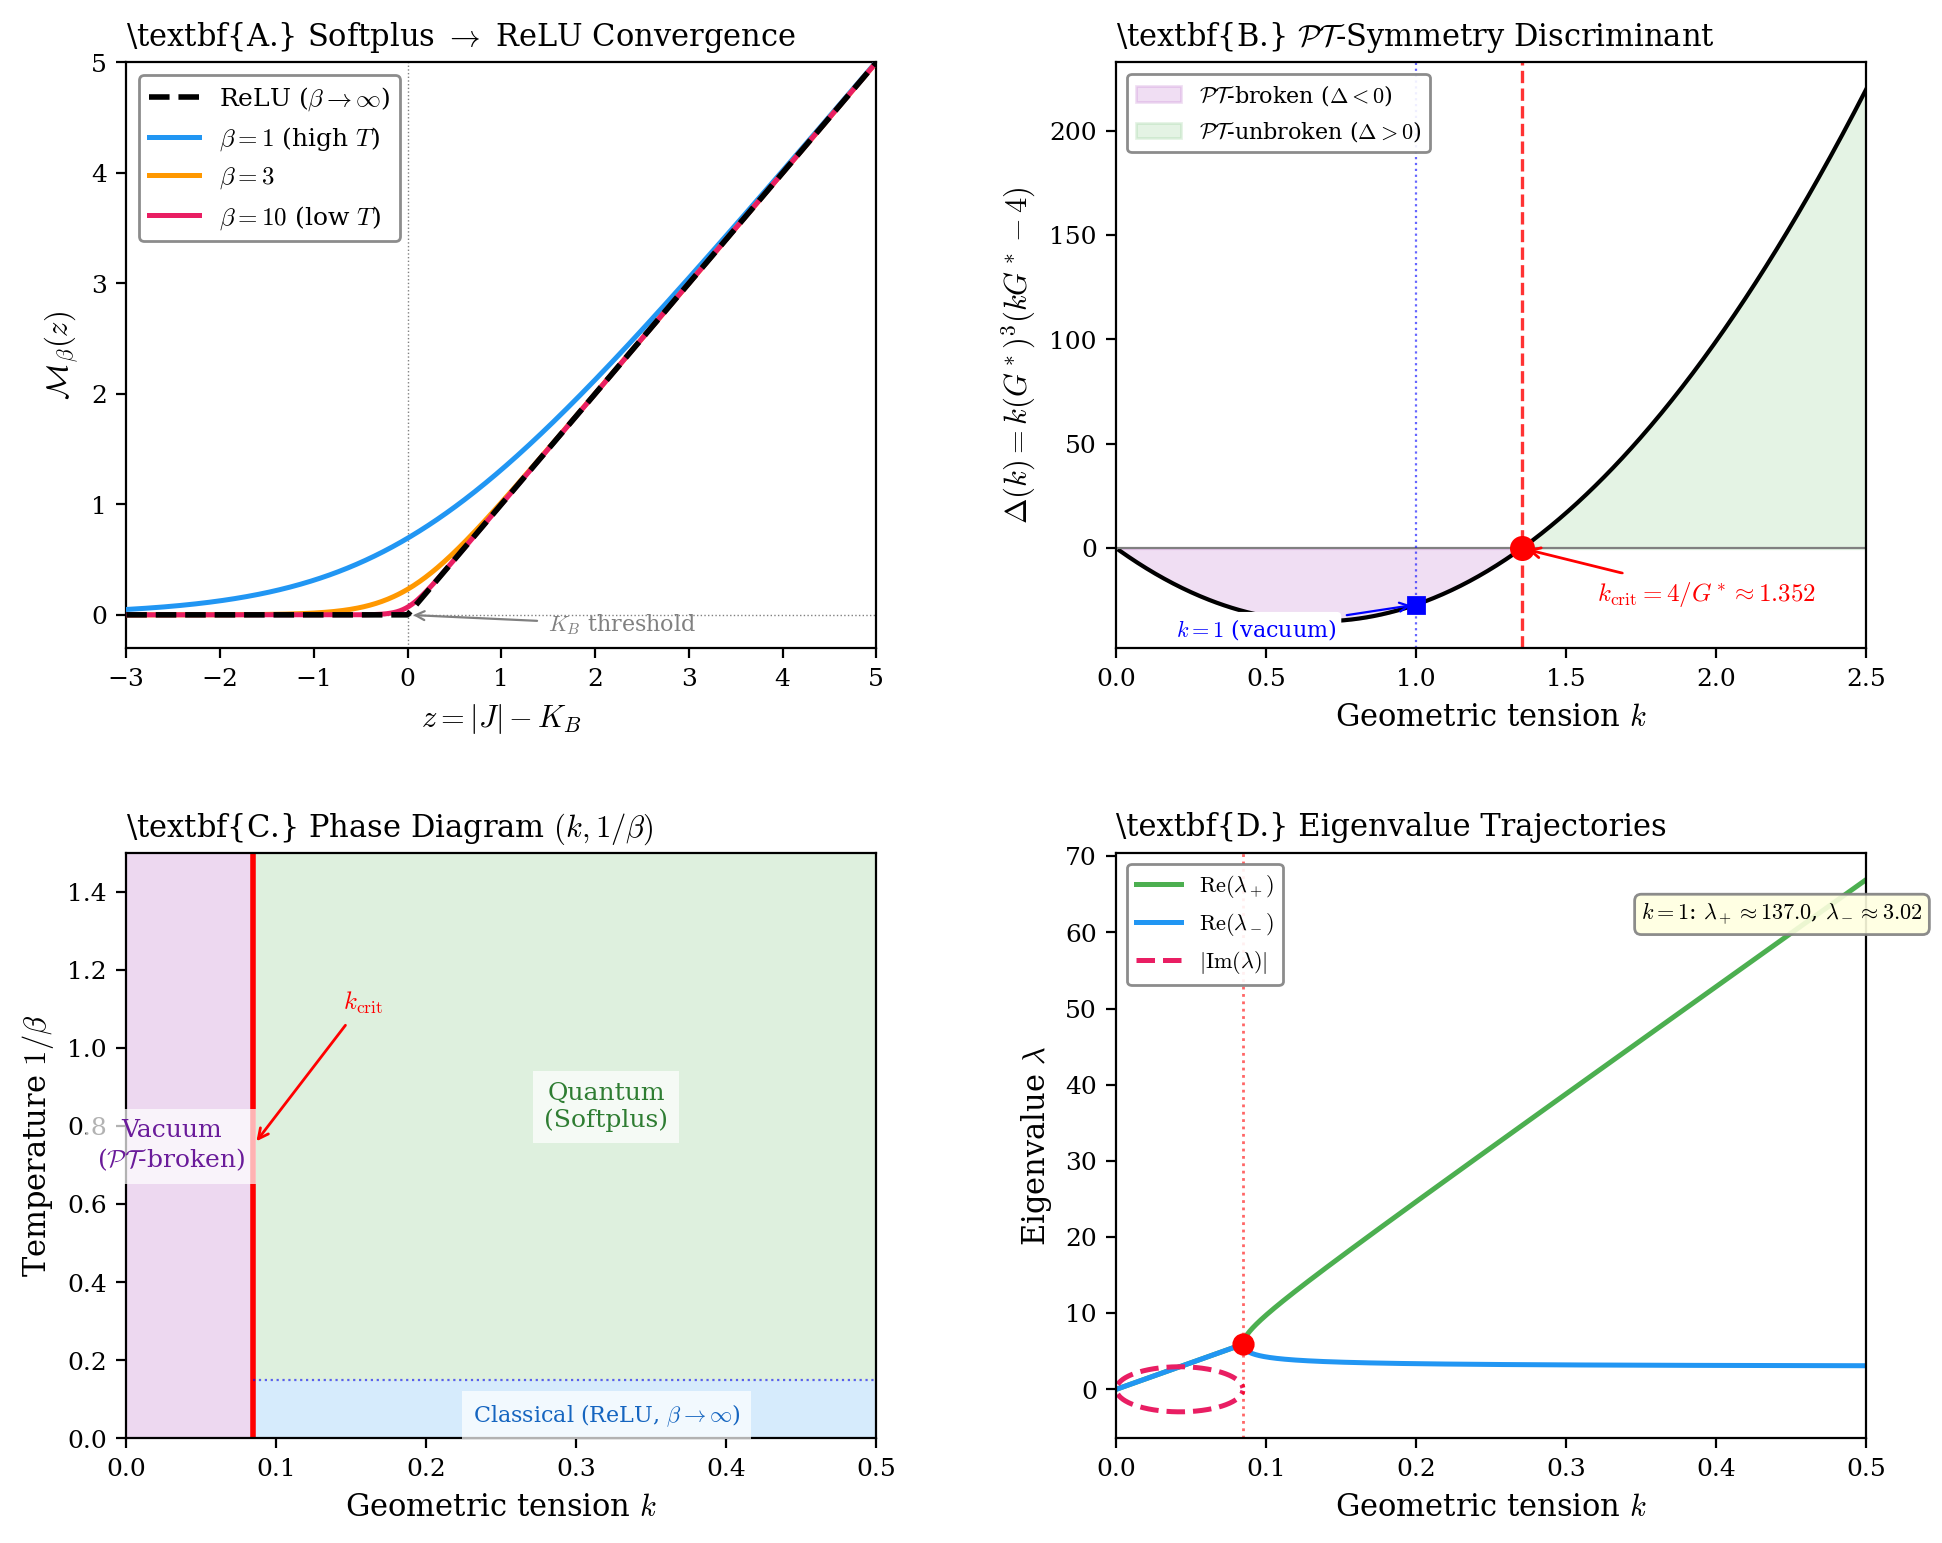
\includegraphics[width=0.95\textwidth]{figures/FTD_Softplus_ReLU.png}
    \caption{\textbf{The Softplus-ReLU phase structure.} \textbf{(A)} The Softplus $\Man_\beta(z)$ at three temperatures, converging mathematically to ReLU as $\beta \to \infty$. \textbf{(B)} The discriminant $\Delta(k)$ in the $n=1$ sector, locating the $\PT$-boundary exactly at $k_{\text{crit}} = 4/\G \approx 1.352$. \textbf{(C)} The $(k, 1/\beta)$ phase diagram mapped in the $n=16$ sector ($k_{\text{crit}} = 1/(4\G) \approx 0.085$), denoting the physical vacuum resting at $k = 1$. \textbf{(D)} Eigenvalue trajectories ($n=16$) tracking $k$ variations; notably at $k = 1$, eigenvalues split strictly to $\lambda_+ \approx 137.04$ and $\lambda_- \approx 3.02$.}
    \label{fig:phase}
\end{figure}

%===============================================================================
\section{Implications and Falsifiable Predictions}
\label{sec:predictions}
%===============================================================================

\subsection{For Mathematical Physics}

The uniqueness theorem (Theorem~\ref{thm:uniqueness}) establishes a new characterization of the Softplus function: it is the unique smooth activation satisfying monotonicity, convexity, asymptotic linearity, and single-species fermionic singularity structure. This result is independent of FTD and may be of interest in the broader study of activation functions in statistical mechanics and information theory.

\subsection{For Lattice Gauge Theory}

The spectral representation (Theorem~\ref{thm:spectral}) provides algebraic constraints on any lattice theory with $n = 16$ physical degrees of freedom and lemniscatic regularization: $\lambda_+\lambda_- = 16(\G)^3$ and $\lambda_+ + \lambda_- = 16(\G)^2$, with the coupling extracted via $\det/\Tr = \G$.

\subsection{Falsification Criteria}

\begin{center}
\renewcommand{\arraystretch}{1.3}
\begin{tabular}{lp{8cm}}
\toprule
\textbf{Claim} & \textbf{Falsifying Observation} \\
\midrule
Uniqueness (Thm.~\ref{thm:uniqueness}) & Evidence that the physical manifestation operator violates one of Axioms M1 through M4 \\
Spectral (Thm.~\ref{thm:spectral}) & Precision $\alpha^{-1}$ inconsistent with $\lambda_+ = 137.036\ldots$ at a threshold exceeding 10 ppm \\
$\PT$ boundary (Thm.~\ref{thm:pt_transition}) & Lattice simulation showing $\Delta = 0$ at $\xi \neq 4$ \\
Critical exponent & Observation of $\nu \neq 1/2$ in a 0-dimensional $\PT$-symmetric matrix model \\
\bottomrule
\end{tabular}
\end{center}

%===============================================================================
\section{Conclusion}
%===============================================================================

We have established four formal results connecting the Softplus activation function, the master quadratic of FTD, $\PT$-symmetry breaking, and Wilsonian renormalization:

\begin{enumerate}[noitemsep]
    \item The Softplus is the unique manifestation operator satisfying four physically motivated axioms. The proof uses a conformal substitution $w = e^{\beta z}$ that maps the analyticity strip to the punctured plane, reducing the problem to showing that the only entire function compatible with the asymptotic constraints is identically zero (Liouville). This result is the strongest contribution of the paper and is independent of FTD.
    \item The FTD master quadratic admits a spectral representation as a canonical $2 \times 2$ Frobenius companion matrix with trace $nc^2$ and determinant $nc^3$, where $n = 16$ (lattice degrees of freedom) and $c = \G$ (lemniscate-alpha coupling). The eigenvalue ratio depends only on $c$, not on $n$; the physical significance of this decoupling remains an open question.
    \item $\PT$-symmetry breaking at $\xi_{\text{crit}} = knc = 4$ partitions the spectrum into real (physical) and complex (vacuum) domains, with exact mean-field exponent $\nu = 1/2$.
    \item The Softplus temperature $\beta$ and the Wilsonian RG scale $\mu$ provide structurally analogous descriptions of UV mode suppression, with $\beta \to \infty$ (ReLU) corresponding to the IR ground state and finite $\beta$ (Softplus) corresponding to the thermally active UV theory.
\end{enumerate}

The Softplus-ReLU duality, read literally, says that the manifestation of matter from void is a finite-temperature phase transition, where the zero-temperature limit produces a sharp classical boundary between existence and non-existence. This confirms that the fermionic Grand Potential does not merely govern statistical mechanics; it dictates the fundamental algorithmic logic gates of discrete lattice gauge theory.

\vspace{2em}
\hrule
\vspace{1.5em}

\begin{thebibliography}{99}

\bibitem{cpaci-tani2026_Zenodo}
W. J. cpaci-tani III,
``Gauge Couplings from Discrete Spacetime Geometry,''
\textit{Foundational Ternary Dynamics Research}, Zenodo (January 2026).

\bibitem{Landau1980}
L. D. Landau and E. M. Lifshitz,
\textit{Statistical Physics, Part 1},
Butterworth-Heinemann, 3rd ed. (1980).

\bibitem{Bender1998}
C. M. Bender and S. Boettcher,
``Real spectra in non-Hermitian Hamiltonians having $\mathcal{PT}$ symmetry,''
\textit{Phys.\ Rev.\ Lett.}\ \textbf{80}, 5243 (1998).

\bibitem{Wilson1974}
K. G. Wilson and J. Kogut,
``The renormalization group and the $\epsilon$ expansion,''
\textit{Phys.\ Rep.}\ \textbf{12}, 75 (1974).

\bibitem{Glorot2011}
X. Glorot, A. Bordes, and Y. Bengio,
``Deep sparse rectifier neural networks,''
\textit{Proc.\ AISTATS}\ \textbf{15}, 315 (2011).

\bibitem{Dugas2001}
C. Dugas, Y. Bengio, F. B\'{e}lisle, C. Nadeau, and R. Garcia,
``Incorporating second-order functional knowledge for better option pricing,''
\textit{Advances in Neural Information Processing Systems}\ \textbf{13} (2001).

\bibitem{Bak1987}
P. Bak, C. Tang, and K. Wiesenfeld,
``Self-organized criticality: An explanation of the $1/f$ noise,''
\textit{Phys.\ Rev.\ Lett.}\ \textbf{59}, 381 (1987).

\bibitem{Callan1970}
C. G. Callan,
``Broken scale invariance in scalar field theory,''
\textit{Phys.\ Rev.\ D}\ \textbf{2}, 1541 (1970).

\bibitem{KMS1957}
R. Kubo,
``Statistical-mechanical theory of irreversible processes. I.,''
\textit{J.\ Phys.\ Soc.\ Japan}\ \textbf{12}, 570 (1957);
P. C. Martin and J. Schwinger,
``Theory of many-particle systems. I.,''
\textit{Phys.\ Rev.}\ \textbf{115}, 1342 (1959).

\bibitem{Kapusta2006}
J. I. Kapusta and C. Gale,
\textit{Finite-Temperature Field Theory: Principles and Applications},
Cambridge University Press, 2nd ed. (2006).

\end{thebibliography}

\end{document}
